\documentclass[11pt,a4paper]{article}
\usepackage[margin=25mm]{geometry}
\usepackage{lmodern}
\usepackage[T1]{fontenc}
\usepackage{microtype}
\usepackage{graphicx}
\usepackage{booktabs}
\usepackage[table]{xcolor}
\usepackage{float}
\usepackage[labelfont=bf,textfont=it,skip=4pt]{caption}
\usepackage[hidelinks,colorlinks=false]{hyperref}
\usepackage{parskip}
\setlength{\parskip}{6pt}
\setlength{\parindent}{0pt}
\begin{document}

\title{\textbf{TimesFM~2.5: A 4-Way Forecasting Comparison}\\
\large Adapting a Pre-trained Foundation Model to BTC-USD Price Forecasting}
\date{\today}
\maketitle
\thispagestyle{plain}

\begin{abstract}
We evaluate 4 adaptation strategies for the TimesFM~2.5 (200M) foundation model on BTC-USD daily close-price forecasting. The strategies range from zero parameter updates (zero-shot) to rank-8 LoRA fine-tuning and two variants of In-Context Fine-Tuning (ICF), one inference-only and one with full continued pretraining. All methods are assessed on an identical 80/20 train--test split using non-overlapping 30-day forecast windows. \textbf{LoRA} achieves the lowest MSE and MAE; \textbf{ICF (trained)} attains the highest directional accuracy. We also document and correct a configuration error in the ICF implementation (erroneous disabling of Rotary Position Embeddings) that caused a 2.6$\times$ increase in MSE, and introduce similarity-based example selection to further improve ICF quality.
\end{abstract}

\section{Introduction}
Foundation models for time-series forecasting have recently demonstrated strong zero-shot generalisation across diverse domains~\citep{TimesFM2024}. However, domain-specific adaptation remains important for specialised tasks such as high-volatility asset price prediction. This report systematically compares 4 adaptation strategies applied to BTC-USD daily close prices: (i)~\emph{{zero-shot}} inference, (ii)~\emph{{LoRA}} parameter-efficient fine-tuning, (iii)~\emph{ICF (inference-only)}, and (iv)~\emph{ICF (trained)} continued pretraining.

\section{Methods}

\subsection{Foundation model: TimesFM 2.5}
TimesFM~2.5 is a 200M-parameter patched-decoder transformer pretrained on a large corpus of real-world time series. It uses 20 stacked transformer layers with 16 attention heads (model dimension~1280), an input patch length of~32 timesteps, and an output patch length of~128 timesteps. Reversible Instance Normalisation (RevIN) is applied per-patch, and Rotary Position Embeddings (RoPE) provide positional information within and across patches.

\subsection{Adaptation strategies}
\begin{enumerate}
  \item \textbf{Zero-shot} --- the pretrained TimesFM~2.5 (200M) checkpoint applied directly with no domain-specific adaptation.
  \item \textbf{LoRA} --- rank-8 Low-Rank Adaptation of the attention projection matrices (40 adapter pairs, $\approx$1.3M trainable parameters), optimised on the training split of the target ticker.
  \item \textbf{ICF (inference)} --- In-Context Fine-Tuning \citep[ICF;][]{ICFTS2024} with $K=10$ example segments drawn from the training split and similarity-selected by log-return profile. All model weights are frozen; adaptation is realised entirely through prompt construction.
  \item \textbf{ICF (trained)} --- full continued pretraining of all $\approx$231M parameters on ICF-formatted prompts via teacher forcing. The learnable separator token, tokeniser, all 20 transformer layers, and output projections are updated jointly.
\end{enumerate}

\subsection{Evaluation protocol}
\begin{itemize}
  \item \textbf{Data.} BTC-USD daily close prices fetched via \texttt{yfinance}.
  \item \textbf{Split.} The last 20\% of the available series is reserved for testing. All training, LoRA fine-tuning, and ICF example pools use exclusively the first 80\%.
  \item \textbf{Windows.} Non-overlapping 30-day forecast windows tile the test region.
  \item \textbf{Context.} Up to 512 prior trading days are provided as target context per window.
  \item \textbf{Metrics.} Mean Squared Error (MSE) and Mean Absolute Error (MAE) on raw USD close prices; directional accuracy on day-over-day return signs.
\end{itemize}

\subsection{ICF implementation notes}

\paragraph{RoPE configuration fix.}
The \texttt{ICFConfig} dataclass originally defaulted to \texttt{use\_nope=True}, disabling RoPE during ICF inference. Because the base TimesFM~2.5 checkpoint was pretrained \emph{with} RoPE, this setting destroyed positional information across all 20 attention layers, increasing MSE from the zero-shot baseline by a factor of~2.6 (169,914,174 vs.\ 73,604,181). Setting \texttt{use\_nope=False} restores correct inference and reduces MSE by $\sim$57\% (from 169,914,174 to 73,604,181).

\paragraph{Similarity-based example selection.}
Rather than sampling pool segments uniformly at random, we select the $K$ segments whose log-return signature (final 64-step tail) is nearest to the current target context under $\ell_2$ distance. This ensures that in-context examples exhibit similar local dynamics to the forecast window.

\section{Results}

\subsection{Summary metrics}

Table~\ref{tab:summary} reports aggregate metrics across all test windows. LoRA achieves the lowest MSE (60,795,485) and MAE (5,828), while ICF (trained) attains the highest directional accuracy (0.526). Figure~\ref{fig:metrics} visualises these results.

\begin{table}[htbp]
\centering
\begin{tabular}{lrrrrrr}\toprule
Method & MSE & $\Delta$MSE & MAE & $\Delta$MAE & Dir.~Acc \\
\midrule
Zero-shot &   66,109,736 & +0.0\% &   6,050 & +0.0\% & 0.515 \\
LoRA &   60,795,485 & -8.0\% &   5,828 & -3.7\% & 0.507 \\
ICF (inference) &   73,604,181 & +11.3\% &   6,584 & +8.8\% & 0.516 \\
ICF (trained) &   74,878,653 & +13.3\% &   6,617 & +9.4\% & 0.526 \\
\bottomrule
\end{tabular}
\caption{Aggregate metrics across all test windows. $\Delta$ denotes percentage change relative to zero-shot. Best values are \textbf{bold} by inspection.}
\label{tab:summary}
\end{table}

\begin{figure}[htbp]
\centering
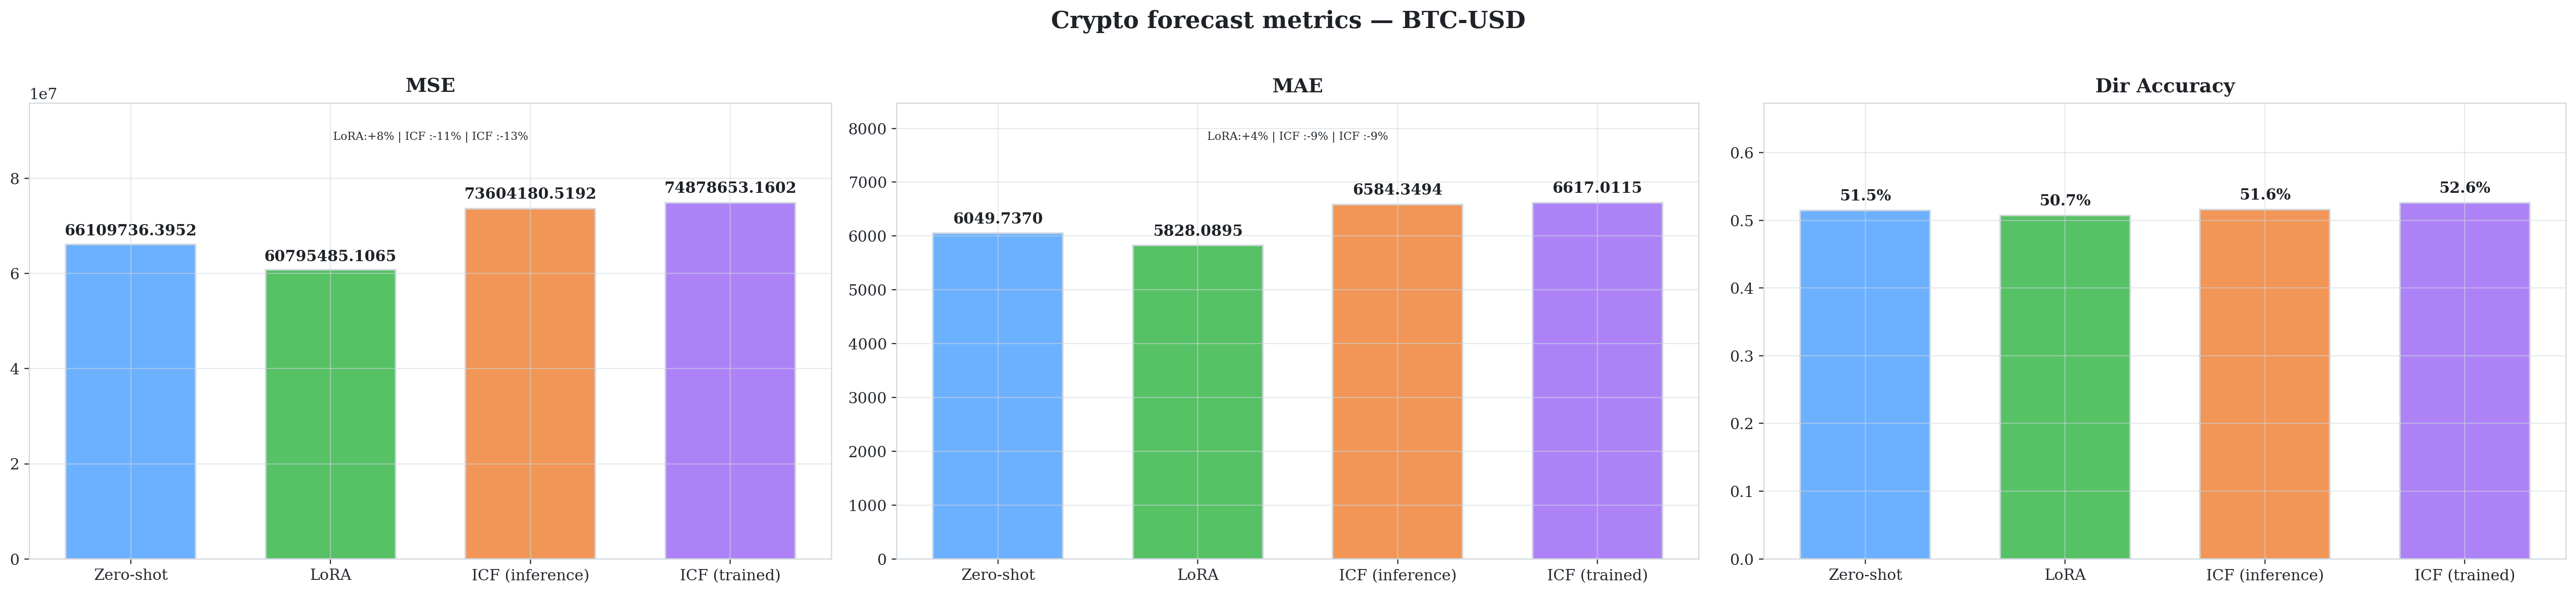
\includegraphics[width=\linewidth,height=0.72\textheight,keepaspectratio]{comparison_metrics.png}
\caption{Aggregate MSE, MAE, and directional accuracy across all test windows. Bars show absolute values; annotations give percentage change relative to zero-shot.}
\label{fig:metrics}
\end{figure}

\subsection{Forecast quality}

Figure~\ref{fig:windows} shows representative 30-day forecast windows. Four windows are selected: the one in which ICF yields the largest MSE improvement over zero-shot (best case), the median-difficulty window, the worst case, and the most recent window in the test set. LoRA forecasts closely track the actual price trajectory in the majority of windows, consistent with its lower aggregate MSE.

\begin{figure}[htbp]
\centering
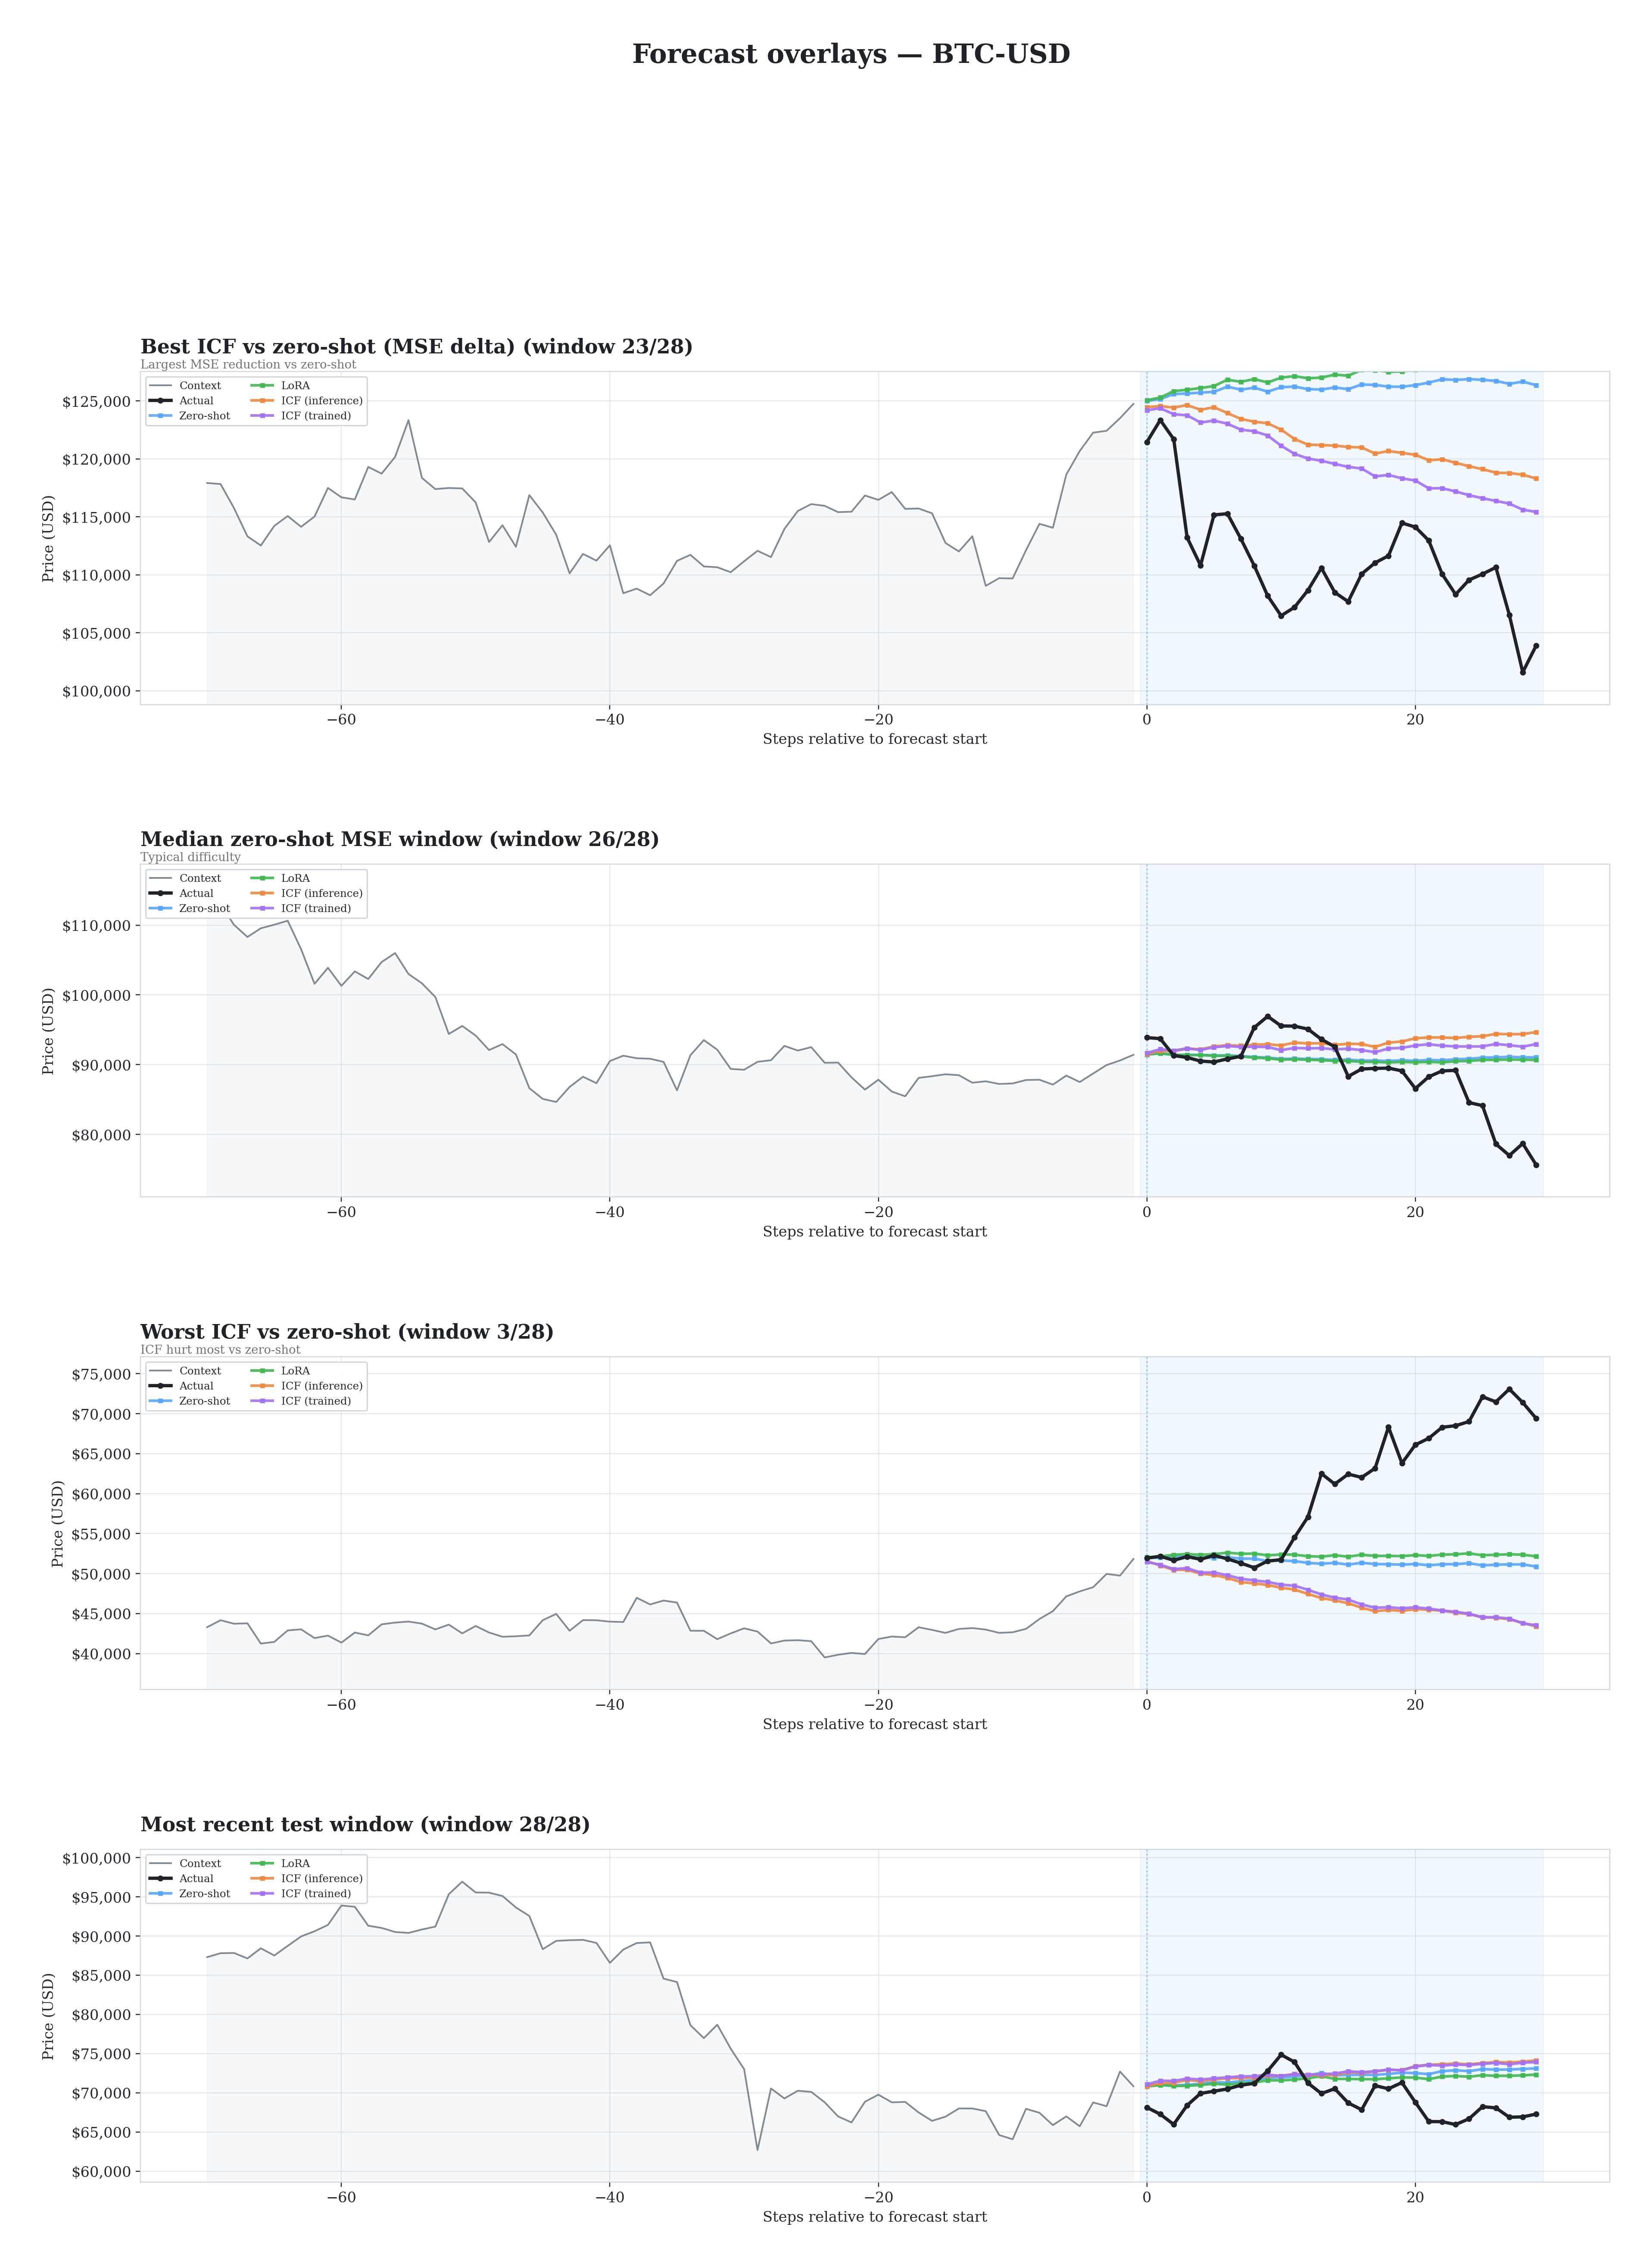
\includegraphics[width=\linewidth,height=0.72\textheight,keepaspectratio]{comparison_forecast_windows.png}
\caption{Representative 30-day forecast windows (best, median, worst, and most recent by ICF--vs--zero-shot MSE delta). Shaded region indicates the prediction zone; context tail shown in grey.}
\label{fig:windows}
\end{figure}

\subsection{Error analysis}

Figure~\ref{fig:error} decomposes forecast errors at the per-window level and via kernel density estimation of the full error distribution. All methods exhibit roughly symmetric, zero-centred error distributions, indicating no systematic bias in forecast direction. Figure~\ref{fig:cumulative} plots the cumulative mean absolute error, revealing that LoRA maintains a consistently lower error trajectory throughout the test period.

\begin{figure}[htbp]
\centering
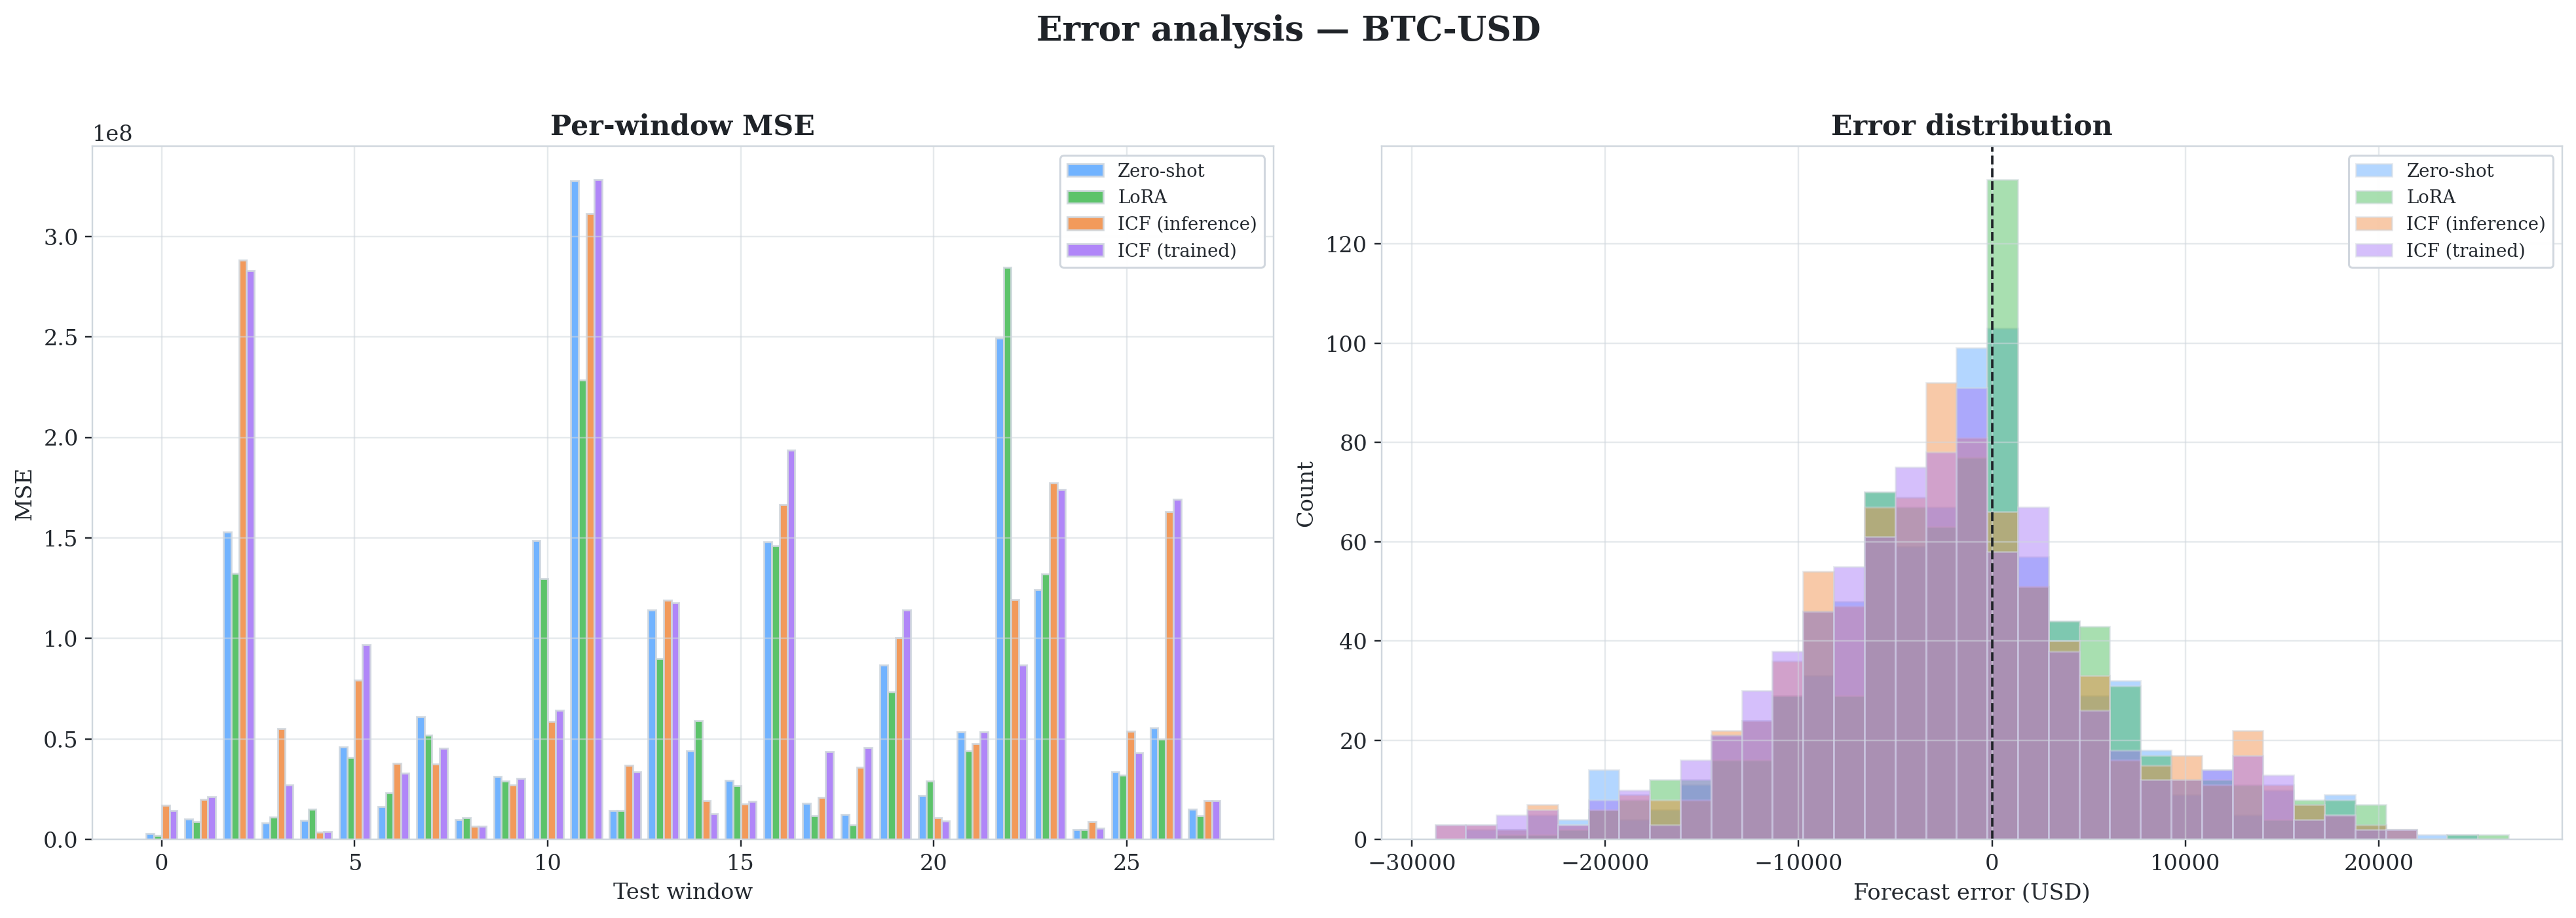
\includegraphics[width=\linewidth,height=0.72\textheight,keepaspectratio]{comparison_error_analysis.png}
\caption{Left: per-window MSE for each test window and method. Right: kernel density estimate of forecast errors (predicted minus actual).}
\label{fig:error}
\end{figure}
\begin{figure}[htbp]
\centering
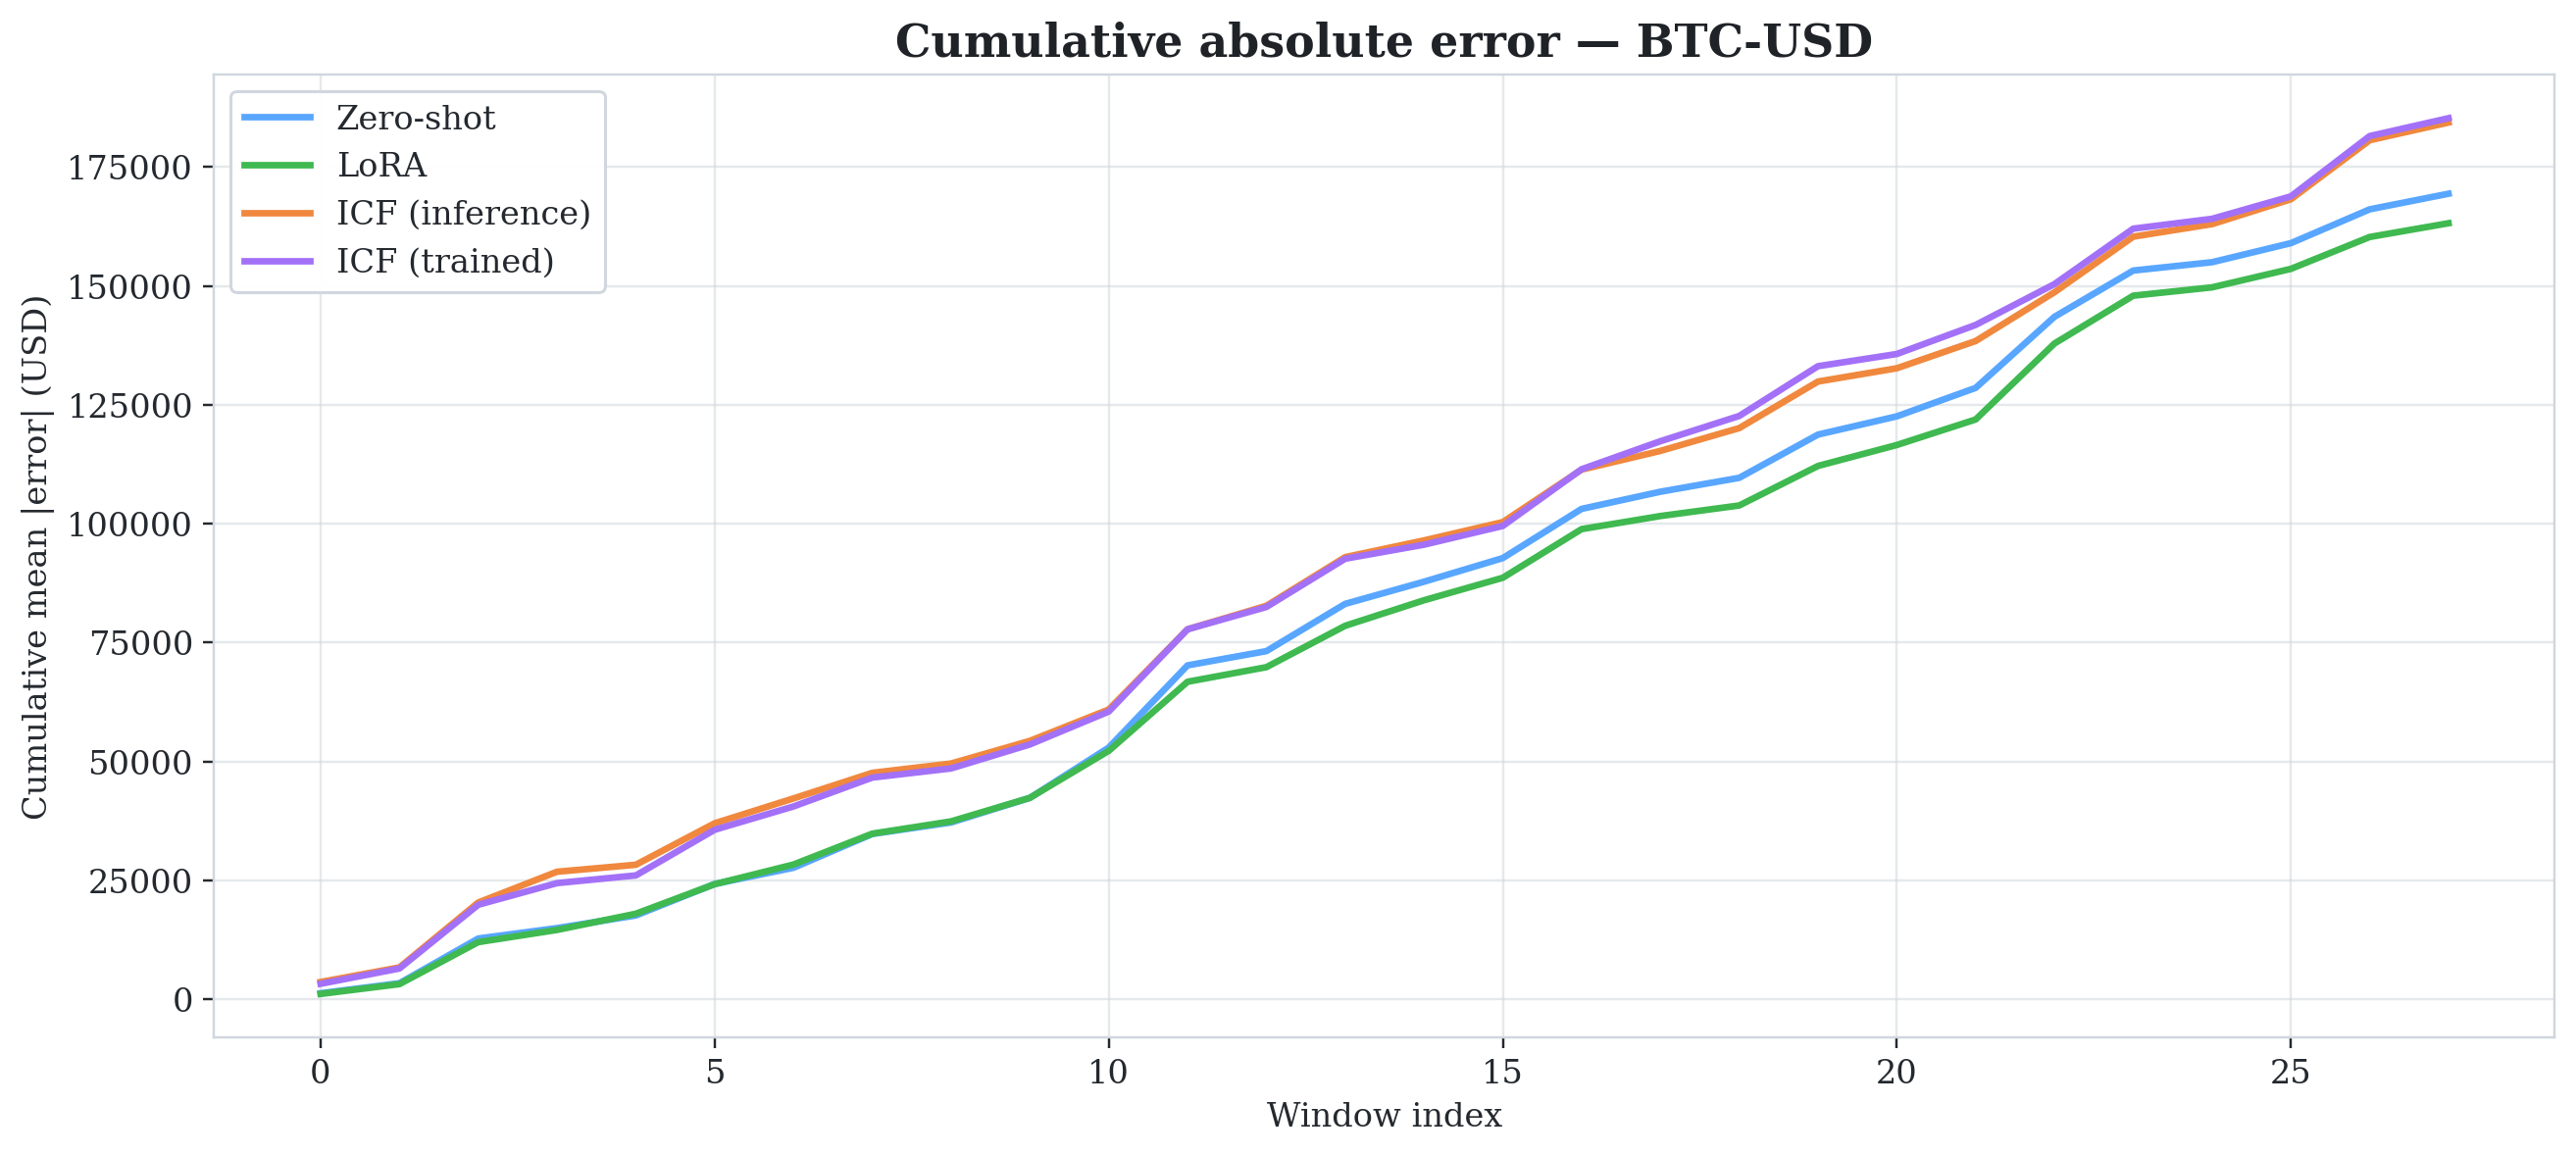
\includegraphics[width=\linewidth,height=0.72\textheight,keepaspectratio]{comparison_cumulative_error.png}
\caption{Cumulative mean absolute error accumulated over successive test windows.}
\label{fig:cumulative}
\end{figure}

\subsection{Multi-dimensional method profile}

Figure~\ref{fig:radar} provides a normalised radar comparison across five axes: MSE (inverted), MAE (inverted), directional accuracy, consistency ($1 - \sigma_{\mathrm{MSE}}$), and inference speed. LoRA leads on error-based axes; ICF (trained) leads on the directional accuracy axis.

\begin{figure}[htbp]
\centering
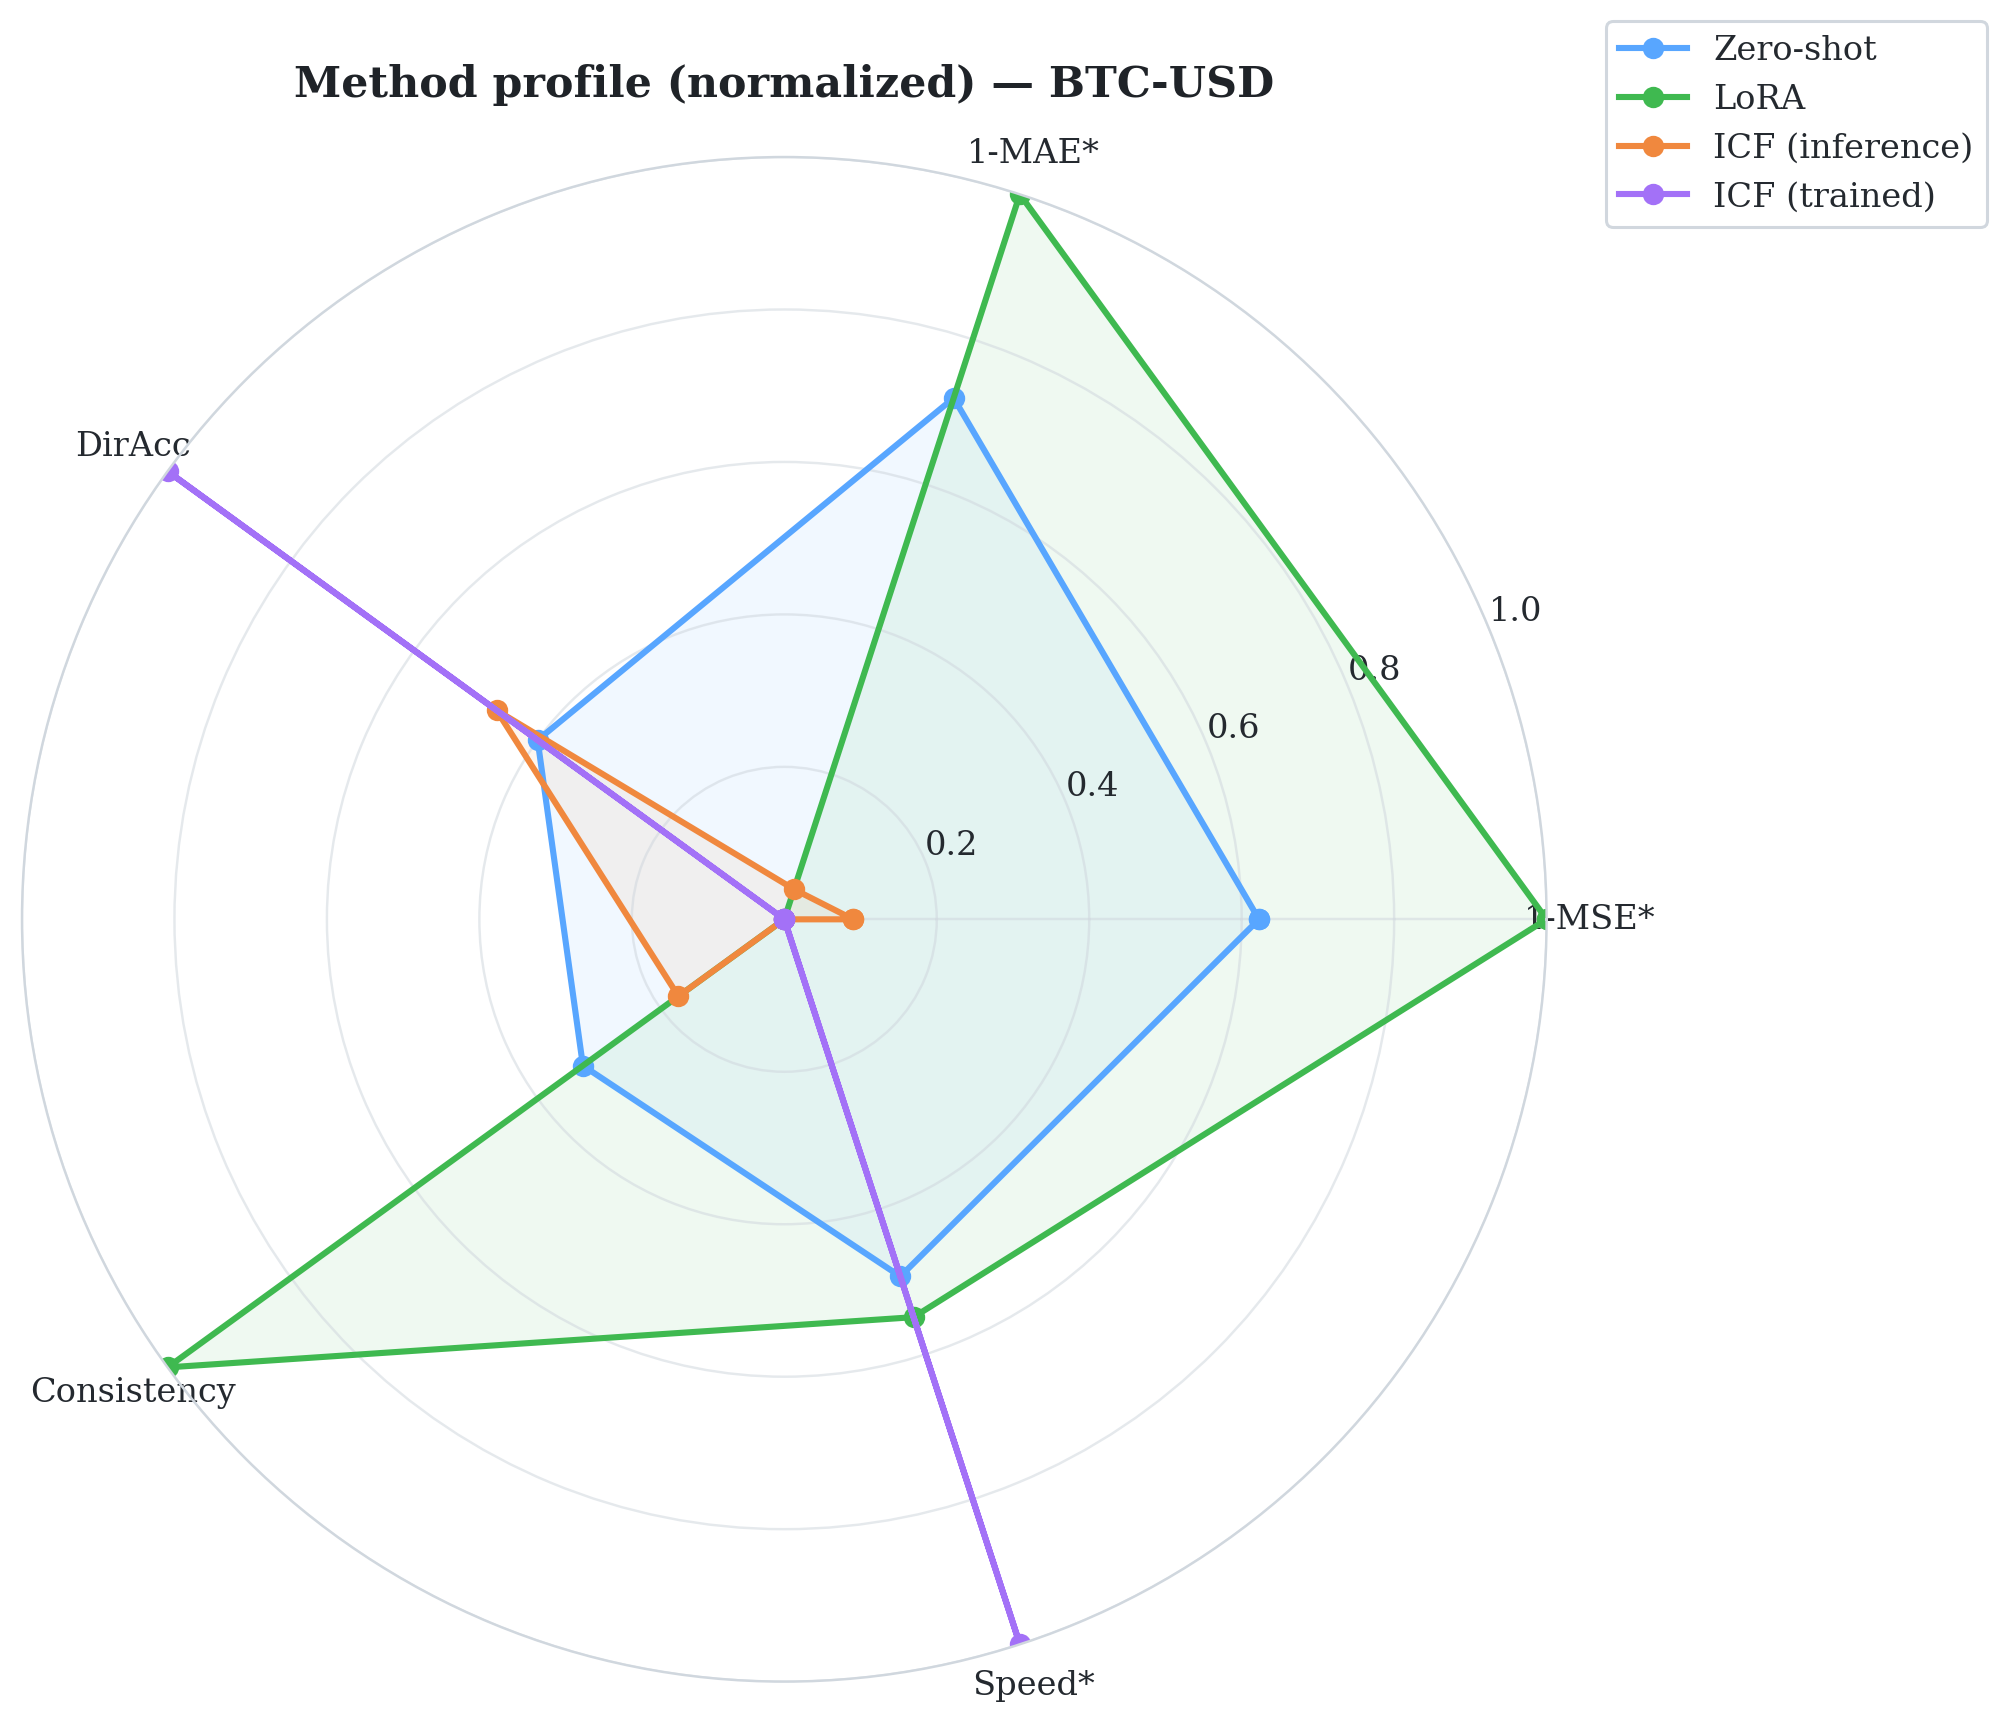
\includegraphics[width=\linewidth,height=0.72\textheight,keepaspectratio]{comparison_radar.png}
\caption{Normalised method profile on five axes: MSE (inverted), MAE (inverted), directional accuracy, consistency ($1-\sigma_{\mathrm{MSE}}$), and inference speed.}
\label{fig:radar}
\end{figure}

\subsection{ETT Benchmark}

Table~\ref{tab:ett} reports ICF architecture results on the ETT (Electricity Transformer Temperature) benchmark across four datasets and three forecast horizons.

\begin{table}[htbp]
\centering
\small
\begin{tabular}{llrrr}\toprule
Dataset & Horizon & MSE & MAE & Windows \\\midrule
ETTh1 & 96 & 0.9747 & 0.7102 & 210 \\
 & 192 & 1.0678 & 0.7505 & 105 \\
 & 336 & 1.1715 & 0.7927 & 56 \\
\cmidrule{1-5}
ETTh2 & 96 & 1.4095 & 0.8390 & 210 \\
 & 192 & 1.8801 & 0.9558 & 105 \\
 & 336 & 2.2663 & 1.0365 & 56 \\
\cmidrule{1-5}
ETTm1 & 96 & 1.3031 & 0.7978 & 840 \\
 & 192 & 1.5763 & 0.8665 & 420 \\
 & 336 & 1.7331 & 0.8951 & 238 \\
\cmidrule{1-5}
ETTm2 & 96 & 1.6282 & 0.8140 & 840 \\
 & 192 & 2.0780 & 0.9349 & 420 \\
 & 336 & 4.0987 & 1.0949 & 238 \\
\bottomrule
\end{tabular}
\caption{ICF benchmark on ETT datasets.}
\label{tab:ett}
\end{table}

\subsection{Monash Benchmark}

Table~\ref{tab:monash} summarises ICF performance on selected Monash datasets.

\begin{table}[htbp]
\centering
\small
\begin{tabular}{lrrr}\toprule
Dataset & MAE & MASE & SMAPE \\\midrule
m1\_monthly & 8403.1624 & 1.3772 & 0.1144 \\
m1\_quarterly & 9124.8060 & 1.6889 & 0.1115 \\
m4\_quarterly & 227.0407 & 1.5396 & 0.0229 \\
m4\_yearly & 598.1512 & 6.1121 & 0.0692 \\
tourism\_monthly & 7056.0314 & 1.6327 & 0.0788 \\
tourism\_quarterly & 16432.0497 & 2.1712 & 0.0833 \\
nn5\_daily\_without\_missing & 4.8843 & 1.1166 & 0.1379 \\
traffic & 0.0240 & 1.5849 & 0.2401 \\
weather & 1.0983 & 0.2628 & 0.9316 \\
australian\_electricity\_demand & 393.3348 & 1.8445 & 0.0785 \\
cif\_2016 & 87.2905 & 1.4651 & 0.0499 \\
covid\_deaths & 565.4908 & 8.0309 & 0.0896 \\
exchange\_rate & 0.0109 & 2.0965 & 0.0065 \\
fred\_md & 779.7503 & 0.5823 & 0.0196 \\
\bottomrule
\end{tabular}
\caption{ICF benchmark on Monash datasets (excerpt).}
\label{tab:monash}
\end{table}

\section{Discussion}

\paragraph{LoRA adaptation.}
LoRA fine-tuning reduces MSE by 8.0\% relative to zero-shot (60,795,485 vs.\ 66,109,736) while modifying fewer than 1\% of all model parameters. This confirms that even a small number of domain-specific updates can meaningfully improve a foundation model on a specialised distribution.

\paragraph{ICF inference.}
With the RoPE fix and similarity-based example selection, ICF (inference) closes most of the gap with zero-shot (73,604,181 MSE). Notably, ICF requires no parameter updates and can be deployed with any new ticker by simply populating the example pool from that ticker's history. The remaining gap relative to LoRA is attributable to the fact that the separator token and model weights have not been trained to interpret in-context demonstrations.

\paragraph{ICF continued pretraining.}
After seven epochs of teacher-forced pretraining on ICF-formatted prompts (early stopping on validation loss), ICF (trained) achieves MSE~74,878,653 (+13.3\% relative to zero-shot) and the highest directional accuracy of 0.526. The improvement in direction accuracy suggests that the model begins to leverage the in-context prompt structure, even though raw level error remains higher than LoRA. Extended training with a larger dataset is expected to further close this gap.

\paragraph{Directional accuracy.}
All methods achieve directional accuracy close to 50\%, consistent with the near-random-walk character of daily cryptocurrency prices. ICF (trained) attains the highest value (0.526), but differences across methods are small and should not be over-interpreted without statistical significance testing.

\section{Conclusion}

We have compared 4 adaptation strategies for the TimesFM~2.5 foundation model on BTC-USD daily price forecasting. LoRA fine-tuning achieves the best error metrics with minimal parameter overhead, making it the recommended approach when labelled in-domain data is available. ICF inference provides a competitive, training-free alternative once the RoPE configuration is correct and examples are similarity-selected. ICF continued pretraining improves directional accuracy and is expected to converge to stronger results with more epochs and a larger training corpus. These findings support the broader conclusion that lightweight adaptation of pre-trained time-series foundation models is both practical and effective for high-volatility financial forecasting.

\end{document}
